\documentclass[11pt]{article}
\usepackage[margin=1in]{geometry}
\usepackage{amsmath,amssymb}
\usepackage{graphicx}
\usepackage{hyperref}
\usepackage{listings}
\usepackage{xcolor}
\usepackage{tikz}
\usetikzlibrary{arrows.meta,positioning,calc}

\definecolor{codegreen}{rgb}{0,0.6,0}
\definecolor{codegray}{rgb}{0.5,0.5,0.5}
\definecolor{codepurple}{rgb}{0.58,0,0.82}
\definecolor{backcolour}{rgb}{0.95,0.95,0.92}

\lstdefinestyle{mystyle}{
    backgroundcolor=\color{backcolour},   
    commentstyle=\color{codegreen},
    keywordstyle=\color{magenta},
    numberstyle=\tiny\color{codegray},
    stringstyle=\color{codepurple},
    basicstyle=\ttfamily\footnotesize,
    breakatwhitespace=false,         
    breaklines=true,                 
    captionpos=b,                    
    keepspaces=true,                 
    numbers=left,                    
    numbersep=5pt,                  
    showspaces=false,                
    showstringspaces=false,
    showtabs=false,                  
    tabsize=2
}
\lstset{style=mystyle}

\title{\textbf{MIT 6.390 Introduction to Machine Learning} \\ \LARGE Lab 8: Representation Learning \& Latent Space Evolution \\ \Large \textit{A Deep Dive into Neural Concept Formation}}
\author{Aditya Sengupta, Professor Manolis Kellis, \& Professor Shen Shen}
\date{Spring 2026}

\begin{document}
\maketitle

\section{Introduction: The Representation Problem}

To understand modern Deep Learning, we must first understand the ``Representation Problem.'' In early machine learning paradigms (which we explored in the first half of this course), we explicitly designed hand-crafted features. For example, to classify an image of a dog, a human engineer might write code to detect edges, compute color histograms, and identify shapes like ``ears'' or ``snouts.'' For text classification, we traditionally rely on \textbf{Bag of Words} or \textbf{TF-IDF} (Term Frequency-Inverse Document Frequency) vectors, which count the occurrences of specific words in a vocabulary of size $V$.

While mathematically sound, these raw representations are highly problematic:
\begin{enumerate}
    \item \textbf{High Dimensionality:} A vocabulary might contain 100,000 words. A single document is an incredibly sparse 100,000-dimensional vector.
    \item \textbf{Lack of Semantic Structure:} In a raw TF-IDF space, the word \textit{``dog''} and the word \textit{``puppy''} correspond to entirely different, orthogonal mathematical axes. The raw data structure has absolutely no concept of synonyms, context, or semantic similarity. 
    \item \textbf{Non-Linear Separability:} Real-world data distributions are heavily entangled. A simple linear classifier (like Logistic Regression) cannot easily draw a hyperplane separating ``Science'' articles from ``Art'' articles if their vocabulary usages overlap significantly.
\end{enumerate}

\begin{figure}[htbp]
    \centering
    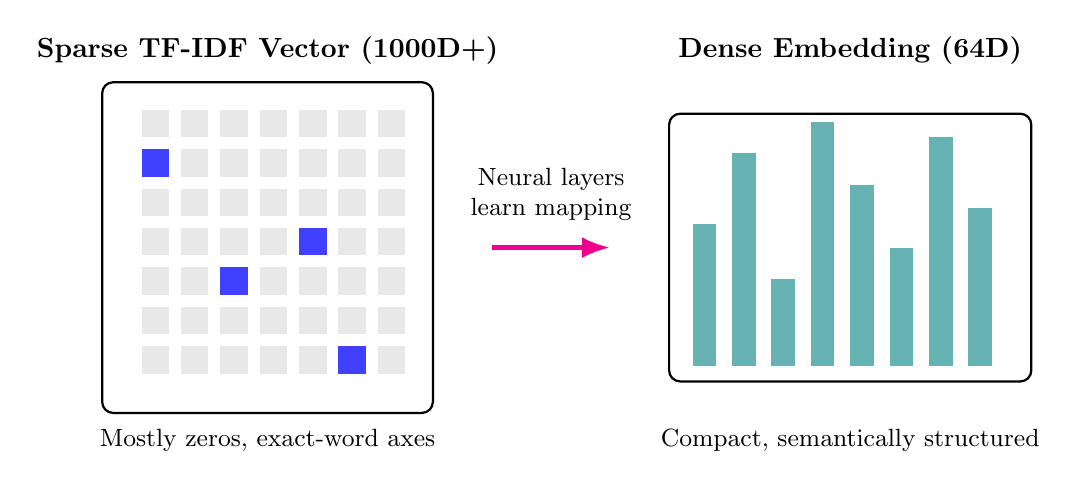
\begin{tikzpicture}[>=Latex, every node/.style={font=\small}]
        % Left side: sparse TF-IDF
        \draw[rounded corners, thick] (0,0) rectangle (4.2,4.2);
        \node[font=\bfseries] at (2.1,4.6) {Sparse TF-IDF Vector (1000D+)};
        \foreach \y in {0.5,1.0,...,3.5} {
            \foreach \x in {0.5,1.0,...,3.5} {
                \fill[gray!18] (\x,\y) rectangle +(0.35,0.35);
            }
        }
        \fill[blue!75] (0.5,3.0) rectangle +(0.35,0.35);
        \fill[blue!75] (1.5,1.5) rectangle +(0.35,0.35);
        \fill[blue!75] (2.5,2.0) rectangle +(0.35,0.35);
        \fill[blue!75] (3.0,0.5) rectangle +(0.35,0.35);
        \node[align=center] at (2.1,-0.35) {Mostly zeros, exact-word axes};

        % Right side: dense embedding
        \draw[rounded corners, thick] (7.2,0.4) rectangle (11.8,3.8);
        \node[font=\bfseries] at (9.5,4.6) {Dense Embedding (64D)};
        \foreach \i/\h in {0/1.8,1/2.7,2/1.1,3/3.1,4/2.3,5/1.5,6/2.9,7/2.0} {
            \fill[teal!60] (7.5+0.5*\i,0.6) rectangle +(0.3,\h);
        }
        \node[align=center] at (9.5,-0.35) {Compact, semantically structured};

        % Arrow
        \draw[->, ultra thick, magenta] (4.95,2.1) -- (6.45,2.1);
        \node[align=center, fill=white, inner xsep=10pt, inner ysep=5pt] at (5.7,2.78) {Neural layers\\learn mapping};
    \end{tikzpicture}
    \caption{Conceptual transition from sparse TF-IDF features to dense learned embeddings.}
    \label{fig:tfidf-to-embedding}
\end{figure}

\section{Deep Learning as Representation Learning}

We often treat neural networks purely as complex \textbf{function approximators} $f_\theta: x \to y$ that map inputs to output probabilities. However, the true superpower of deep learning is \textbf{Representation Learning}.

Instead of forcing a linear classifier to solve an impossible puzzle in the raw, messy input space, a neural network uses successive layers of non-linear transformations (such as ReLU activations and weight matrices) to geometrically \textbf{warp, fold, and squash the data space}.

By the time the data reaches the final hidden layer (the ''penultimate'' layer) of the network, the chaotic raw input has been mapped into a dense, lower-dimensional continuous vector space. This learned mathematical space is called the \textbf{Latent Space} or \textbf{Embedding Space}.

In this Latent Space:
\begin{itemize}
    \item \textbf{Proximity represents similarity:} Concepts that are semantically identical (e.g., an article on ``Machine Learning'' and an article on ``Deep Learning'') are physically pulled together into tight clusters by the gradient descent process, even if they don't share exact keywords.
    \item \textbf{Linear properties emerge:} The network morphs the dataset to the point where the different categories become perfectly linearly separable. The final \textit{Softmax} classification layer is ultimately just drawing a simple, flat hyperplane boundary through this newly-organized latent geometry.
\end{itemize}

\section{The Dynamics of Learning}

Neural networks do not magically know how to construct these beautiful geometric manifolds immediately. In this lab, you will not just look at the final model; you will perform an algorithmic ``autopsy'' across time.

\subsection{Epoch 0: The Chaotic Initialization}
Before training begins, PyTorch initializes the weight matrices of your network randomly. If you pass an article through the untrained network, the resulting vector in the latent space is essentially random noise limit. If we plot these untrained embeddings, we will see an interspersed, structureless cloud. The network is completely blind to the underlying concepts.

\subsection{Epochs 1 through 10: Gradient Sculpting}
As we execute Stochastic Gradient Descent (SGD) and compute the Cross-Entropy Loss, backpropagation begins updating the weights. Mathematically, the gradient acts as an attractive/repulsive physical force in the high-dimensional space:
\begin{itemize}
    \item \textbf{Attractive Forces:} Inputs with the same target label are heavily penalized for being far apart. The network updates its weights to map them closer together.
    \item \textbf{Repulsive Forces:} Inputs with different target labels are penalized for crossing decision boundaries, causing the network geometry to stretch and push contradictory classes away from each other.
\end{itemize}

As epochs progress, you will physically watch distinct ``islands'' of knowledge break away from the chaotic center and solidify.

\begin{figure}[htbp]
    \centering
    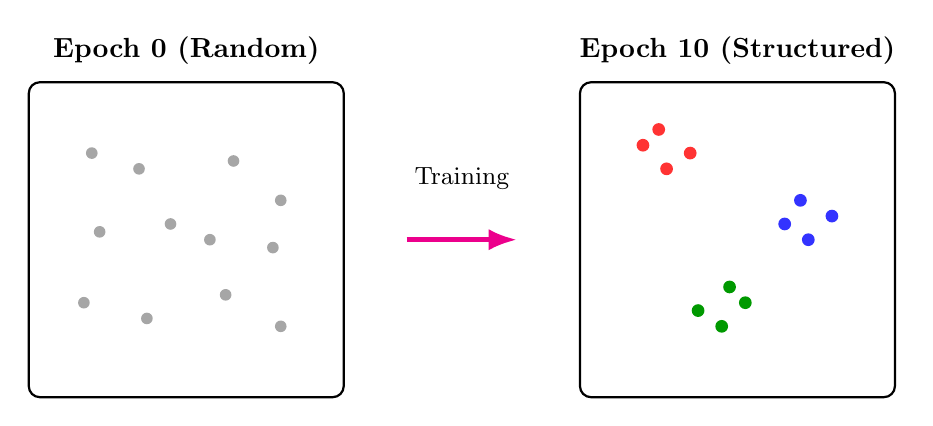
\begin{tikzpicture}[>=Latex, every node/.style={font=\small}]
        % Epoch 0 cloud
        \draw[thick, rounded corners] (0,0) rectangle (4,4);
        \node[font=\bfseries] at (2,4.4) {Epoch 0 (Random)};
        \foreach \p in {(0.8,3.1),(1.4,2.9),(2.6,3.0),(3.2,2.5),(0.9,2.1),(1.8,2.2),(2.3,2.0),(3.1,1.9),(0.7,1.2),(1.5,1.0),(2.5,1.3),(3.2,0.9)} {
            \fill[gray!70] \p circle (2.1pt);
        }

        % Epoch 10 clusters
        \draw[thick, rounded corners] (7,0) rectangle (11,4);
        \node[font=\bfseries] at (9,4.4) {Epoch 10 (Structured)};
        \foreach \p in {(7.8,3.2),(8.1,2.9),(8.4,3.1),(8.0,3.4)} {\fill[red!80] \p circle (2.3pt);} 
        \foreach \p in {(9.6,2.2),(9.9,2.0),(10.2,2.3),(9.8,2.5)} {\fill[blue!80] \p circle (2.3pt);} 
        \foreach \p in {(8.5,1.1),(8.8,0.9),(9.1,1.2),(8.9,1.4)} {\fill[green!60!black] \p circle (2.3pt);} 

        \draw[->, ultra thick, magenta] (4.8,2) -- (6.2,2);
        \node[align=center, fill=white, inner xsep=5pt, inner ysep=5pt] at (5.5,2.78) {Training};
    \end{tikzpicture}
    \caption{Learning dynamics in latent space: unstructured initialization to clustered concept organization.}
    \label{fig:epoch-evolution}
\end{figure}


\begin{figure}[htbp]
    \centering
    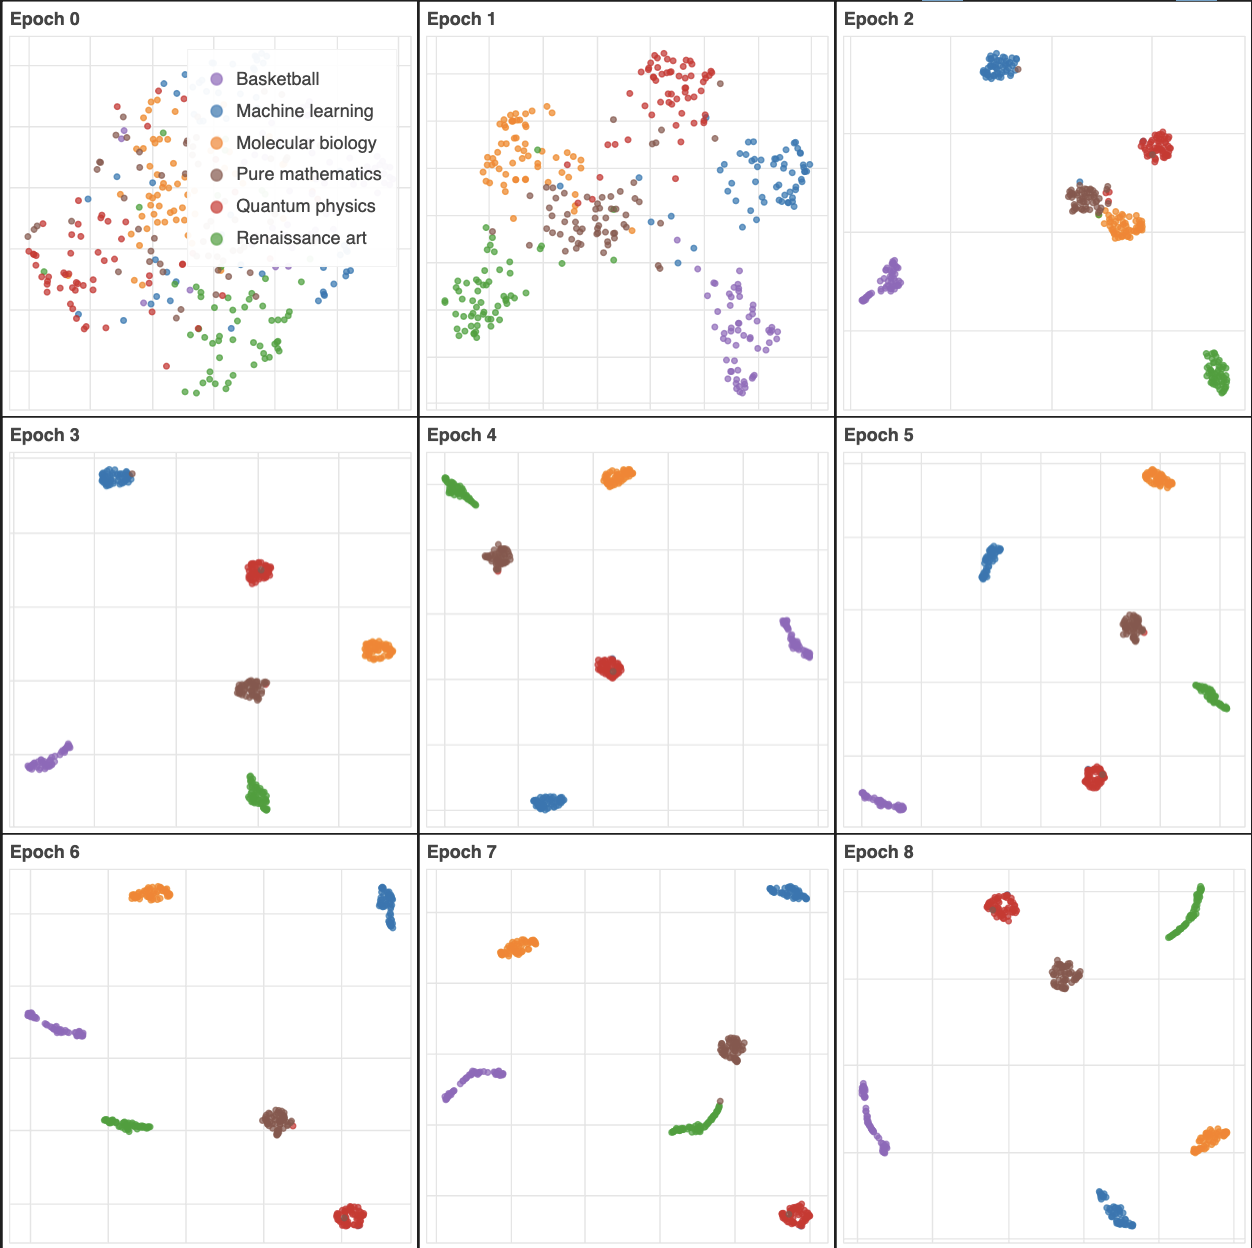
\includegraphics[width=0.5\linewidth]{UMAP-Over-Epochs.png}
    \caption{UMAP trajectories across epochs, showing latent-space organization from initialization to trained structure.}
    \label{fig:umap-over-epochs}
\end{figure}

\section{Visualizing High Dimensions: UMAP \& Mantis}

A core problem in representation learning is that our latent spaces are typically 64, 128, or 1024 dimensions. Human brains cannot comprehend 128-dimensional geometry. 

To solve this, we rely on dimensionality reduction algorithms like \textbf{UMAP (Uniform Manifold Approximation and Projection)}. UMAP mathematically preserves the local neighborhood distances of the 128D space while flattening it down to 2D or 3D for us to visualize on a screen.

\subsection{The Mantis Platform}
To rigorously map the learning trajectory of your model in 3D, you will leverage \href{https://mantis.csail.mit.edu/}{Mantis}, a high-dimensional data visualization and exploration suite extensively used in computational biology and latent mapping at MIT. 

\begin{figure}[htbp]
    \centering
    \includegraphics[width=0.9\linewidth]{Mantis-UI.png}
    \caption{Mantis interface for exploring high-dimensional embeddings projected with UMAP.}
    \label{fig:mantis}
\end{figure}

\clearpage
\section{Lab Activity Walkthrough}

\subsection{Part 1: Training the Feature Extractor}
Your primary objective is to train a multi-layer neural network on a text classification task and freeze snapshots of its latent space at different moments in time.

\begin{enumerate}
    \item Open the primary lab notebook: \texttt{notebooks/part1\_text\_classification.ipynb}.
    \item \textbf{The Dataset:} This notebook dynamically queries the real, live Wikipedia API. It searches for highly complex topics (e.g., ``Quantum Physics'', ``Renaissance Art'', ``Machine Learning'') and downloads the first 150 article abstracts for each. \textit{(You are highly encouraged to modify the \texttt{topics} list in the Python cell to scrape entirely different subjects that you find interesting!)}
    \item \textbf{The Baseline Features:} The text is passed through a \texttt{TfidfVectorizer} to convert the raw strings into our massive, messy, 1000-dimensional baseline vectors.
    \item \textbf{The Training Loop:} Execute the training loop. Pay close attention to the fact that we are running the model for 10 \textit{Epochs} (full passes over the dataset).
\end{enumerate}

\subsection{Part 2: The Neural Network ``Hook''}
Study the PyTorch architecture defined in the notebook:

\begin{lstlisting}[language=Python]
class TextClassifier(nn.Module):
    def __init__(self, vocab_size, hidden_dim, num_classes):
        super(TextClassifier, self).__init__()
        self.fc1 = nn.Linear(vocab_size, 256)
        self.relu = nn.ReLU()
        self.fc2 = nn.Linear(256, hidden_dim) # Bottleneck representation
        self.classifier = nn.Linear(hidden_dim, num_classes)
        self.embeddings = None # Hook initialization
        
    def forward(self, x):
        out = self.relu(self.fc1(x))
        out = self.fc2(out) # Shape: [Batch, hidden_dim]
        # ---> THE EXTRACTION HOOK <---
        self.embeddings = out.detach().cpu().numpy() 
        out = self.relu(out)
        out = self.classifier(out)
        return out
\end{lstlisting}

Notice what is happening here! During the \texttt{forward} pass, right before the data hits the final \texttt{self.classifier} layer, we intercept the \texttt{out} tensor. We copy its exact numerical state and save it into \texttt{self.embeddings}. 

Every single epoch, our loop invokes model evaluations and appends these captured 64-dimensional arrays into a massive list. 

\subsection{Part 3: CSV Generation and Mantis Upload}
Once the model finishes training, the notebook runs a cell to export a widely structured DataFrame containing your raw text, the article titles, and 11 unique columns: \texttt{embedding\_epoch\_0}, \texttt{embedding\_epoch\_1}, ... \texttt{embedding\_epoch\_10}.

\begin{enumerate}
    \item Download the resulting \texttt{text\_analysis\_wikipedia\_mantis.csv} file to your computer.
    \item Navigate your web browser to \href{https://mantis.csail.mit.edu/}{Mantis}.
    \item Upload your \texttt{.csv} file into the platform.
    \item In Mantis, select \texttt{embedding\_epoch\_0} as the primary coordinate vector space to render via UMAP. Color the points using the \texttt{categoric} metric.
    \item Observe the lack of structure.
    \item Now, switch the vector space to \texttt{embedding\_epoch\_10}. Watch the points dynamically animate and fly to their newly learned, deeply structured coordinates.
\end{enumerate}

\clearpage
\section{Assignment Questions}

\subsection{Conceptual Representation Questions}

\textbf{Q1 (2 points).} Explain in your own words why raw TF-IDF vectors are computationally cumbersome and semantically limited compared to dense neural embeddings. 

\vspace{4cm}

\textbf{Q2 (2 points).} Why must we explicitly extract and save the latent representations \textit{before} the final softmax or linear classifier layer rather than just looking at the final model prediction probabilities?

\vspace{4cm}

\textbf{Q3 (3 points).} As training progresses from Epoch 0 to Epoch 10, explain theoretically what transformations you expect to observe regarding the Euclidean distance between a Wikipedia article on ``Quantum Physics'' and one on ``Renaissance Art'' versus ``Machine Learning'' and ``Pure Mathematics'' within the embedding space?

\vspace{4cm}

\textbf{Q4 (2 points).} In Epoch 0, the model weights are instantiated randomly. What does the distribution of points look like on the UMAP reduction grid, and conceptually, are there any inherent structures visible before backpropagation?

\vspace{4cm}

\subsection{Coding and Architecture Questions}

\textbf{Q5 (3 points).} We use a custom PyTorch model class to extract and save the embeddings inline via \texttt{self.embeddings = out.detach().cpu().numpy()}. \\
Why is the \texttt{.detach()} method absolutely critical in this assignment? What would physically happen to memory and the PyTorch \texttt{autograd} (automatic differentiation) graph if this method was omitted inside our multi-epoch loop?

\vspace{4cm}

\textbf{Q6 (2 points).} If a student sets an aggressively high learning rate (e.g., $lr=0.5$ via the Adam Optimizer) in the Colab notebook, how might the plotted UMAP space behave across Epoch 1 through Epoch 5 in contrast to a well-behaved network using the default $lr=0.001$? 

\vspace{4cm}

\textbf{Q7 (2 points).} When fetching the Wikipedia API dynamically, you can easily change the subjects. Can you think of two Wikipedia topics that might "fool" the neural network into creating overlapping latent clusters at Epoch 10, instead of cleanly separated islands? Briefly justify your answer.

\vspace{4cm}

\begin{center}
\textbf{End of Assignment.} 
\end{center}

\end{document}
